%% inicio, la clase del documento es especificacion.cls
\documentclass{especificacion}
\usepackage[onelanguage, commentsnumbered, linesnumbered, boxed, ruled]{algorithm2e}
\usepackage{pdfpages}
\usepackage{amsfonts}
\usepackage{amssymb}
\usepackage{array}
\usepackage{longtable}
\usepackage{float}
\usepackage{setspace}
\usepackage{listings}

\lstset{ %
    language=Java, % lenguaje
    basicstyle=\bfseries\ttfamily,
    keywordstyle=\color{blue},
    commentstyle=\color{brown},
    backgroundcolor=\color{gray!10},
    showstringspaces=false
}

%% datos generales y para la tapa
\titulo{Documento de especificaci�n de requisitos}
\subtitulo{Herramienta para la optimizaci�n de redes de distribuci�n de agua potable}
\author{Gabriel Gonzalo Alexander Sanhueza Fuentes}


%% inicio de documento
\begin{document}

%% crea la tapa
\maketitle

\adddevelopment{Gabriel Sanhueza Fuentes}{Administrador, Analista, Dise�ador, Implementador y Tester.}{gsanhueza15@alumnos~.utalca.cl}

\addcounterpart{Jimmy H. Guti�rrez-Bahamondes}{Cliente/Profesor gu�a}{}
\addcounterpart{Jimmy H. Guti�rrez-Bahamondes}{Cliente/Profesor co-gu�a}{}

\addrevision{0.1}{07/09/2019}{Primer borrador}
\addrevision{0.2}{30/09/2019}{Rellenar arquitectura l�gica}
\addrevision{0.3}{05/09/2019}{Agregar diagramas de clases}
\addrevision{0.4}{12/12/2019}{Agregado diagrama de secuencia y m�dulos}
\addrevision{0.5}{13/12/2019}{Agregado detalle de anotaciones}
\addrevision{1}{30/01/2020}{Modificada definici�n de anotaciones}
\addrevision{1.1}{06/06/2020}{Modificada definici�n de anotaciones nuevamente para satisfacer requisitos nuevos. \singlespace Cambio en dise�o de interfaces.}


\RevisionHistoryPage


%% indices
\tableofcontents
\listoffigures
%\listoftables

%% abstract

%WRITE HERE
\chapter{Introducci�n}
El proyecto que se desarrollara consiste en la creaci�n de una herramienta que haga uso de algoritmos metaheur�sticos para tratar y minimizar problemas existentes en redes de distribuci�n de agua potable.

Este proyecto solo abarcara dos problemas existentes dentro de las redes de distribuci�n de agua potable.

Para el desarrollo de este proyecto se usar�n librer�as ya existentes con el fin de reducir el tiempo de desarrollo. Estas librer�as son epanet2.dll, desarrollada en c, y JNA, librer�a en java para funciones nativas.


\section{Prop�sito del Sistema}

El proyecto consiste en el desarrollo de un sistema que permite simular y buscar soluciones a problemas presentes en las redes de distribuci�n de agua potable haciendo uso de algoritmos metaheur�sticos. Adicionalmente, el sistema es dise�ado de tal forma que pueda ser extendido a�adiendo nuevos problemas, algoritmos u operadores.
\section{Alcance del proyecto}

Al final del periodo de desarrollo la herramienta contara con las siguientes prestaciones.

\begin{itemize}
    \item	El sistema permitir� la carga y la visualizaci�n de la red gr�ficamente.
    \item	El sistema solo resolver� dos clases de problemas de optimizaci�n, uno mono-objetivo y el otro multiobjetivo. El problema mono-objetivo ser� el de los costos de inversi�n. En cuanto al problema multiobjetivo, este ser� el de los costos energ�ticos y el n�mero de encendidos y apagado de las bombas.  
    \item	El sistema �nicamente contara con dos algoritmos implementados los cuales ser�n el algoritmo gen�tico y NSGA-II. El algoritmo gen�tico ser� el usado para tratar el problema mono-objetivo, mientras que NSGA-II ser� aplicado al multiobjetivo.
    \item	El sistema permitir� visualizar y guardar las soluciones de los algoritmos en un archivo.
    \item	El sistema permitir� que el usuario agregue nuevos algoritmos, operadores o problemas sin tener que modificar la interfaz de usuario.
\end{itemize}

Este proyecto no contempla la creaci�n de la red por lo que estas deber�n ser ingresadas como entradas al programa. 

Adem�s, esta herramienta �nicamente podr� ser ocupada en equipos cuyo sistema operativo sea Windows debido a que se realizan llamadas a librer�as nativas.

\section{Contexto}

Este sistema ser� desarrollado utilizando el lenguaje de programaci�n java. Debido a que este es un lenguaje ampliamente utilizado y que cuenta con un gran soporte y comunidad que lo utilizan.

Como motor de c�lculo para llevar a cabo las simulaciones se utilizar� una librer�a desarrollada en c, que cuenta con funciones para llevar a cabo simulaciones de redes de agua potable. El nombre de esta librer�a es epanet2.dll. Las funciones que incorpora esta librer�a se encuentran explicadas en~\cite{Rossman2017}.

Desde lenguaje se realizar�n llamadas a librer�as nativas usando la librer�a JNA existente en java. Esta librer�a cuenta con las clases y m�todos necesarios para poder acoplar este sistema a la librer�a epanet2.dll desarrollada en c y que ser� usada como motor de c�lculo para llevar a cabo las simulaciones.
Puesto que una de las funcionalidades del sistema es permitir la ejecuci�n de algoritmos metaheur�sticos, se toma como base la arquitectura presentada por el framework JMetal.

JMetal es un framework para la optimizaci�n multiobjetivo con metaheur�sticas. Su arquitectura inicial~\cite{Durillo2010} involucraba una serie de problemas y dificultaban la realizaci�n de ciertas acciones que eran recurrentes. Adem�s, esta no hacia uso de las novedades incorporadas por Java como los gen�ricos. Es por esto, que posteriormente fue redise�ada, haciendo uso de patrones de dise�o, principios de la programaci�n orientada a objetos y aprovechando las caracter�sticas del lenguaje Java. Este redise�o se presenta en~\cite{Nebro2015}.

El contexto en el que se desenvolver� este sistema ser� en ambientes universitario, de investigaci�n y en el ambiente laboral. 

\section{Definiciones, Acr�nimos y Abreviaturas}

NSGA-II: Non-dominated Sorting Genetic Algorithm
%% genera las referencias
\bibliography{refs}
\chapter{Dise�o arquitect�nico}

\section{Arquitectura F�sica}

La arquitectura f�sica del software a desarrollar consiste en la arquitectura monol�tica. Puesto que es un programa de escritorio cuya persistencia de datos se realiza en el mismo equipo del usuario que est� ejecutando la aplicaci�n y no necesita interacci�n con otros sistemas o equipos. En la Figura \ref{fig:arquitectura_fisica} se puede ver una imagen que representa la arquitectura.

\begin{figure}[H]
    \centering
    \includegraphics[width=0.5\textwidth]{Capitulo2/assets/arquitectura_fisica.png}
    %%\adjincludegraphics[width=\textwidth, trim={0 0 0 {0.3\height}},clip, rotate = 180]{Capitulo3/assets/matriz_req-u_req-s.eps}
    \caption{Arquitectura f�sica.}
    \label{fig:arquitectura_fisica}
\end{figure}
\section{Arquitectura l�gica}

La arquitectura l�gica que se utilizar� corresponde al patr�n Modelo-Vista-Controlador~\cite{Syromiatnikov2014}. La elecci�n de este patr�n se debe a que permite la separaci�n de la l�gica de negocio y la vista presentada al usuario logrando de esta manera una aplicaci�n altamente mantenible y con una mejor escalabilidad. El diagrama que representa la arquitectura usada para el desarrollo se puede ver en la Figura \ref{fig:arquitectura_logica}.  

\begin{figure}[H]
    \centering
    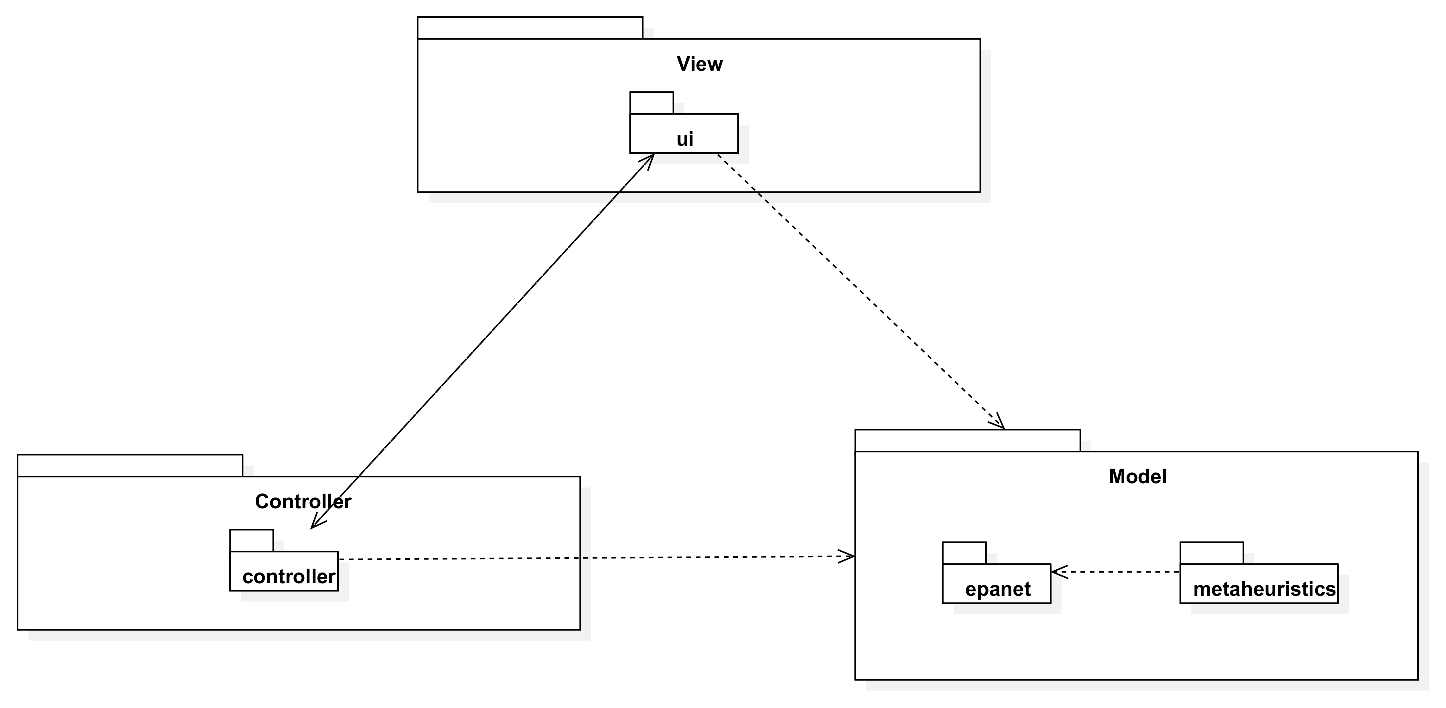
\includegraphics[width=\textwidth]{Capitulo2/assets/arquitectura_logica.eps}
    \caption{Arquitectura l�gica.}
    \label{fig:arquitectura_logica}
\end{figure}

En el diagrama presentado en la Figura \ref{fig:arquitectura_logica} se presencia la divisi�n de la aplicaci�n en tres capas. La capa Vista se encarga de la interacci�n con el usuario y de la interfaz de usuario. La capa Controlador se encarga de responder a los eventos de los usuarios y solicitar informaci�n a la capa de modelo. La capa Modelo contiene la informaci�n y la l�gica fundamental de la aplicaci�n en un formato adecuado para interactuar con las dem�s capas. Esta �ltima capa, tambi�n se encarga de la ejecuci�n de los algoritmos y la interacci�n con la librer�a nativa EpanetToolkit.

La capa Modelo se divide principalmente en dos componentes. Estos componentes son:

\paragraph{Componente Metaheur�sticas (\textit{Metaheuristics}):}
Modulo que contiene los algoritmos, operadores, los tipos de soluci�n permitidos y los problemas que ser�n abarcados durante el desarrollo del proyecto. 

\paragraph{Componente Hidr�ulico (EPANET):}
El m�dulo hidr�ulico posee las clases necesarias para cargar los archivos de red (inp) y generar una representaci�n de ellos a trav�s de una serie de clases. Este m�dulo tambi�n se encarga de guardar la representaci�n de una red ya modificada en un archivo inp para que pueda ser usado por el programa EPANET. Las simulaciones hidr�ulicas ser�n realizadas usando la librer�a epajava. Esta librer�a realiza las llamadas nativas a la EpanetToolkit. La librer�a epajava puede ser descargada en el repositorio de git ubicado en https://github.com/jhawanet/epajava .

\chapter{Dise�o detallado}
Durante esta secci�n se presenta el dise�o de la aplicaci�n de manera m�s detallada, acompa�ado junto con una series de diagramas que describen la funcionalidad o algunas operaciones que realiza el sistema.

\section{Dise�o detallado de m�dulos}

Los componentes que forman la aplicaci�n son el componente de la GUI, el de los Controlladores, el componente de Epanet y el componente Metaheur�sticas. La relaci�n entre los componentes puede ser apreciada en la Figura \ref{fig:diagrama_componentes}.

\begin{figure}[H]
    \centering
    \includegraphics[width=\textwidth]{Capitulo3/assets/diagrama_de_componentes.eps}
    \caption{Diagrama de componentes.}
    \label{fig:diagrama_componentes}
\end{figure}

A continuaci�n, se describe cada uno de los componentes presentados en la Figura \ref{fig:diagrama_componentes}:

\begin{description}
    \item[\textit{GUI (Graphics User Interface)}]	Este componente est� encargado de presentar todas las vistas. Entre las vistas se encuentra la ventana principal de la aplicaci�n, la ventana de configuraci�n de para un problema, la ventana de ejecuci�n de algoritmos y la ventana de resultados.
    \item[\textit{Controller}]	El controlador se encarga de manejar los eventos generados por la \textit{GUI}. Generalmente la relaci�n es uno a uno, es decir, por cada interfaz de usuario hay un controlador. Debido a que la interfaz de usuario est� formada por varios componentes gr�ficos, se da el caso en que cada uno de �stos puede tener su propio controlador. 
    \item[Epanet]	Este componente esta encargada de la lectura y la escritura de archivos de configuraci�n de red (Llamado desde ahora como archivo inp). Este componente cuenta tambi�n con clases que representan una red cargada desde un inp. Estas clases permitir�n editar, durante la ejecuci�n del programa, algunas configuraciones de la red.  Posteriormente, estas configuraciones podr�n ser persistidas generando un nuevo archivo de configuraci�n de red.
    \item[\textit{Metaheuristics}]	Este componente contiene los algoritmos metaheur�sticos, as� como los problemas y los operadores que pueden ser ocupados por los algoritmos.
    \item[epajava.jar]	Esta es una librer�a para la simulaci�n de las redes de agua potable. Esta librer�a permite realizar llamadas nativas a la librer�a de Epanet. Estas llamadas nativas se hacen a trav�s de la librer�a \textit{JNA (Java Native Access)}. Para ocupar la librer�a, esta requiere que se indique el archivo de descripci�n de la red (Archivo inp).
\end{description}


\section{Dise�o de estructura de sistema}

En la Ilustraci�n 4 se muestra un diagrama general de los componentes, sus clases m�s importantes y su interacci�n.En la Figura \ref{fig:diagrama_general} se muestra un diagrama general de los componentes, sus clases m�s importantes y su interacci�n.

\begin{figure}[H]
    \centering
    \includegraphics[width=\textwidth]{Capitulo3/assets/diagrama_general}
    \caption{Diagrama de clases general del sistema.}
    \label{fig:diagrama_general}
\end{figure}


La Figura \ref{fig:diagrama_clase_red} corresponde a un diagrama de clases m�s detallado del componente Epanet.

\begin{figure}[H]
    \centering
    \includegraphics[width=\textwidth]{Capitulo3/assets/class_network.eps}
    \caption{Diagrama de clase de la red.}
    \label{fig:diagrama_clase_red}
\end{figure}


En la Figura \ref{fig:module_metaheuristic}, se presenta el diagrama de clases del componente metaheur�stico. Este fue tomado de~\cite{Nebro2015} y adaptado para ser usado por nuestra aplicaci�n.

\begin{figure}[H]
    \centering
    \includegraphics[width=\textwidth]{Capitulo3/assets/module_metaheuristic.eps}
    \caption{Diagrama de clases del componente \textit{metaheuristic}.}
    \label{fig:module_metaheuristic}
\end{figure}    
\section{Operaci�n del sistema}

A continuaci�n, se presentan una serie de diagramas de secuencia que describen las interacciones entre las clases para ciertas funcionalidades.

En la Figura~\ref{fig:seq_load_visualization}, se presenta la secuencia de tareas que realiza la aplicaci�n desde que es abierta hasta que se visualiza la red.

Luego, en la Figura~\ref{fig:seq_simulation}, se muestra la serie de acciones realizadas para realizar la simulaci�n hidr�ulica utilizando los valores por defecto del archivo de red.

Despu�s, en la \ref{fig:seq_optimization}, se puede observar la interacci�n entre las clases de la aplicaci�n para poder llevar a cabo la resoluci�n de un problema, sea este monoobjetivo o multiobjetivo.

Finalmente, en la Figura~\ref{fig:dia_actividades} se muestra un diagrama de actividades de las operaciones que se pueden llevar a cabo con la aplicaci�n. En est� diagrama de actividades, los nodos amarillos corresponde a la parte del proceso en que se utiliza \textit{Java Reflection API} y \textit{Java Annotation}, los cuales son presentados en el cap�tulo~\ref{cap:reflection_annotation}.

\begin{figure}[H]
    \centering
    \includegraphics[width=0.95\textheight, angle=90]{Capitulo3/assets/sequence_load_visualization_network.eps}
    \caption{Diagrama de secuencia de la carga y visualizaci�n de la red.}
    \label{fig:seq_load_visualization}
\end{figure}

\begin{figure}[H]
    \centering
    \includegraphics[width=0.95\textheight, angle=90]{Capitulo3/assets/sequence_hydraulic_simulation.eps}
    \caption{Diagrama de secuencia de la simulaci�n de la red usando los valores del archivo de configuraci�n de red (inp).}
    \label{fig:seq_simulation}
\end{figure}

\begin{figure}[H]
   \centering
   \includegraphics[width=\textwidth]{Capitulo3/assets/sequence_optimization.eps}
   \caption{Diagrama de secuencia de la optimizaci�n.}
   \label{fig:seq_optimization}
\end{figure}

\begin{figure}[H]
    \centering
    \includegraphics[width=\textwidth]{Capitulo3/assets/d_actividad.eps}
    \caption{Diagrama de actividades}
    \label{fig:dia_actividades}
 \end{figure}
 


\chapter{Dise�o de interfaces}
Durante este cap�tulo se presentan las interfaces que conforman la aplicaci�n.

\section{Interfaz de inicio}
La interfaz de inicio se divide en tres secciones, el men�, el visualizador de red y un apartado para ver los elementos de la red. Para cargar una red debe ir a \textit{File} $>$ \textit{Open}. Para resolver un problema debe ir al men� \textit{Problems} y elegir el problema a resolver. Para ver m�s detalles de un componente de la red, entonces pulse dos veces en componente de la red en el apartado de elementos. Esta interfaz se muestra en la Figura \ref{fig:interfaz_inicio}.

\begin{figure}[H]
    \centering
    \includegraphics[width=\textwidth]{Capitulo4/assets/InterfazInicio.png}
    \caption{Esquema de interfaz de inicio del sistema.}
    \label{fig:interfaz_inicio}
\end{figure}

\section{Interfaz de configuraci�n y descripci�n del problema}
La interfaz de configuraci�n y descripci�n del problema es mostrada cuando el problema tiene par�metros que configurar. La Figura~\ref{fig:interfaz_descripcion_problema} muestra la interfaz de descripci�n del problema a optimizar. La Figura~\ref{fig:interfaz_configuracion_problema} muestra la interfaz para configurar los par�metros del problema.

\begin{figure}[H]
    \centering
    \includegraphics[width=\textwidth]{Capitulo4/assets/InterfazDeConfiguracion1.png}
    \caption{Interfaz de descripci�n del problema.}
    \label{fig:interfaz_descripcion_problema}
\end{figure}

\begin{figure}[H]
    \centering
    \includegraphics[width=\textwidth]{Capitulo4/assets/InterfazDeConfiguracion2.png}
    \caption{Interfaz de configuraci�n del problema.}
    \label{fig:interfaz_configuracion_problema}
\end{figure}

\section{Interfaz de ejecuci�n del experimento}

Esta interfaz es mostrada mientras se lleva a cabo la ejecuci�n del algoritmo. Existen 2 interfaces de ejecuci�n. Una para el problema monoobjetivo y otra para el multiobjetivo. La Figura \ref{fig:interfaz_experimento_monoobjetivo} muestra la interfaz usada cuando el problema es monoobjetivo. Por otro lado, la Figura \ref{fig:interfaz_experimento_multiobjetivo} muestra la interfaz para los problemas multiobjetivos.

Si se presiona el bot�n cancelar, entonces la ejecuci�n del algoritmo ser� detenida.

La pesta�a ``\textit{Chart}'' est� disponible para la interfaz de los problemas multiobjetivos de hasta dos objetivos.

\begin{figure}[H]
    \centering
    \includegraphics[width=\textwidth]{Capitulo4/assets/InterfazDeEjecucion1.png}
    \caption{Interfaz de ejecuci�n del experimento monoobjetivo.}
    \label{fig:interfaz_experimento_monoobjetivo}
\end{figure}

\begin{figure}[H]
    \centering
    \includegraphics[width=\textwidth]{Capitulo4/assets/InterfazDeEjecucion2.png}
    \caption{Interfaz de ejecuci�n del experimento multiobjetivo.}
    \label{fig:interfaz_experimento_multiobjetivo}
\end{figure}

\section{Interfaz de gr�ficos}
Esta interfaz es mostrada cuando se selecciona la pesta�a ``\textit{Chart}''. �sta cuenta con un gr�fico de dos ejes. Si el problema es de un objetivo, entonces el eje vertical corresponde al valor del objetivo despu�s de realizar la evaluaci�n, mientras que el eje horizontal corresponde al n�mero de generaciones. Si el problema tiene dos objetivos, el eje vertical corresponde al primer objetivo y el eje horizontal corresponde al segundo objetivo. La interfaz para problemas monoobjetivos es mostrada en la Figura~\ref{fig:interfaz_grafica_soluciones_mono}, mientras que para el problema multiobjetivo se muestra la interfaz en la Figura~\ref{fig:interfaz_grafica_soluciones_multi}.

\begin{figure}[H]
    \centering
    \includegraphics[scale=0.7]{Capitulo4/assets/grafico_soluciones_monoobjetivo.png}
    \caption{Interfaz de gr�fico de soluciones para problemas monoobjetivos}
    \label{fig:interfaz_grafica_soluciones_mono}
\end{figure}

\begin{figure}[H]
    \centering
    \includegraphics[scale=0.7]{Capitulo4/assets/grafico_soluciones_multiobjetivo.png}
    \caption{Interfaz de gr�fico de soluciones para problemas multiobjetivos}
    \label{fig:interfaz_grafica_soluciones_multi}
\end{figure}

\section{Interfaz de resultados}
La interfaz de resultados es mostrada cuando la ejecuci�n del algoritmo ha terminado exitosamente. Esta interfaz es mostrada en la ventana principal de la aplicaci�n en una nueva pesta�a. Al seleccionar una pesta�a de resultado se activan tres botones como se muestra en la Figura \ref{fig:interfaz_resultados_optimizacion}.

El bot�n ``\textit{Save selected �tem as inp}'' crea un inp para la soluci�n selecciona. Para esto se env�a una copia del objeto Network abierto y la soluci�n al m�todo applySolutionToNetwork, al objeto problema. Este m�todo sustituye en el objeto Network los valores correspondientes indicados en la soluci�n y devuelve nuevamente el objeto Network para poder guardarlo usando un objeto que implementa la interfaz OutputWriter.

El bot�n ``\textit{Save Table}'' guarda todas las soluciones, en dos archivos separados. Uno de estos archivos guarda solamente las variables de decisi�n, y el otro guarda los valores de los objetivos. El nombre de �stos corresponde al dado a trav�s del FileChooser que es mostrado al presionar el bot�n. A este nombre se le agrega el sufijo -FUN, para el archivo con los valores de los objetivos; y -VAR, para el archivo con los valores de las variables de decisi�n.

El bot�n ``\textit{Save Table as Excel}'' exporta la tabla a una planilla Excel.

\begin{figure}[H]
    \centering
    \includegraphics[width=\textwidth]{Capitulo4/assets/InterfazDeResultados.png}
    \caption{Interfaz de resultados de la optimizaci�n}
    \label{fig:interfaz_resultados_optimizacion}
\end{figure}
 
\section{Interfaz de visualizaci�n de configuraciones de la red}
Al seleccionar un componente de la red en la interfaz gr�fica y hacer doble click se abrir� una interfaz que permite ver la configuraci�n por defecto de los componentes de la red. Esta interfaz consiste en mostrar una tabla en donde la primera columna ser� el nombre del atributo de la red y la segunda el valor. Un ejemplo de esta interfaz para un componente de la red se puede visualizar en la Figura \ref{fig:interfaz_visualizacion_configuracion}.

\begin{figure}[H]
    \centering
    \includegraphics[width=\textwidth]{Capitulo4/assets/InterfazDeVisualizacionDeConfiguracionRed.png}
    \caption{Interfaz de visualizaci�n de la configuraci�n de la red.}
    \label{fig:interfaz_visualizacion_configuracion}
\end{figure}
 
\section{Interfaz de ejecuci�n de una red}
Se puede ejecutar una red con su configuraci�n por defecto. Una vez ejecutada la red se puede visualizar en una interfaz los resultados de su ejecuci�n. Este interfaz se muestra en la Figura \ref{fig:interfaz_resultado_simulacion}.
 
\begin{figure}[H]
    \centering
    \includegraphics[width=\textwidth]{Capitulo4/assets/InterfazDeResultadosDeSimulacion.png}
    \caption{Interfaz de resultados de ejecuci�n de simulaci�n hidr�ulica.}
    \label{fig:interfaz_resultado_simulacion}
\end{figure}

Los botones ``\textit{Time series for nodes}'' y ``\textit{Time series for link}'' solo son mostrados cuando la red est� configurada para simular m�s de un periodo de tiempo de simulaci�n.

\chapter{Detalles de implementaci�n}
Una necesidad del sistema es poder a�adir nuevos algoritmos, operadores y problemas. Sin embargo, para hacer uso de �stos desde la interfaz de usuario, ser�a necesario que el implementador modifique manualmente la interfaz. Esto llevar�a una carga extra al implementador al tener que aprender la tecnolog�a necesaria que fue usada para crear la interfaz, la cual para este sistema corresponde a JavaFX. Debido a estas razones, para facilitar el trabajo del implementador se tom� como alternativa usar dos tecnolog�as del lenguaje de Java, las cuales son\textit{ Java Reflection} y\textit{ Java Annotation}.  
El uso que se hace por parte de ellas en el sistema es:

\begin{description}
    \item[\textit{Java Reflection}] Examina las clases durante la ejecuci�n del programa con el fin de construir una interfaz de usuario que permita configurar los valores que ser�n necesarios al momento de crear un objeto de dicha clase.
    \item[\textit{Java Annotation}] Agrega metadatos a los elementos del programa, en este caso a los constructores, que ser�n le�dos a trav�s de la\textit{ Java Reflection API}. Estos metadatos contienen informaci�n del constructor como el nombre de los par�metros que recibe y en el caso de que el par�metro sea un objeto, las alternativas de las clases para crear dicho objeto.
\end{description}

Haciendo uso de estas dos tecnolog�as, se puede reducir esta preocupaci�n, puesto que, estableciendo y siguiendo una convenci�n se puede crear din�micamente una la \textit{GUI} para instanciar nuevos objetos sin conocer su tipo previamente en tiempo de compilaci�n. La convenci�n anteriormente mencionada, consiste en implementar una interfaz, en la cual el constructor indique los par�metros que requiere, los cuales deben estar en un orden determinado, para crear y configurar el algoritmo cuando este sea solicitado a trav�s del m�todo declarado por la interfaz. El nombre de dicha interfaz es \textit{Registrable}.

\section{Uso de \textit{Java Annotation} y \textit{Java Reflection}}
Las anotaciones presentes en el sistema, su finalidad y donde deber�an ser usadas se define a continuaci�n:
\subsection{Anotaciones para los operadores}

\subsubsection{\textit{@DefaultConstructor}}

Indica el constructor que debe ser usado al momento de crear una instancia del operador. Esta anotaci�n recibe un arreglo de \textit{NumberInput}, el cual se define en la siguiente secci�n. El arreglo debe tener la misma cantidad de argumentos que los par�metros del constructor como se muestra en la Figura \ref{fig:constructor_un_parametro} y Figura \ref{fig:constructor_multi_parametro}. 

\begin{figure}[H]
    \centering
    \includegraphics[width=\textwidth]{Capitulo5/assets/ConstructorUnParametro.png}
    \caption{Constructor de un solo par�metro.}
    \label{fig:constructor_un_parametro}
\end{figure}
  
\begin{figure}[H]
    \centering
    \includegraphics[width=\textwidth]{Capitulo5/assets/ConstructorMultiParametro.png}
    \caption{Constructor de un solo par�metro.}
    \label{fig:constructor_multi_parametro}
\end{figure}

Esta anotaci�n solo puede ser usada en un �nico constructor por clase. Usar esta anotaci�n en m�s de un constructor lanzara una excepci�n en tiempo de ejecuci�n. Adicionalmente, el constructor que use esta anotaci�n solo puede tener par�metros de tipo \textit{int} o \textit{double}.

La interfaz gr�fica creada para cada anotaci�n se puede ver en la Figura \ref{fig:interfaz_uniform_selection} y \ref{fig:interfaz_polynomial_mutation}.

\begin{figure}[H]
    \centering
    \includegraphics[width=0.5\textwidth]{Capitulo5/assets/InterfazConfiguracionUniformSelection.png}
    \caption{Interfaz para configurar el operador \textit{UniformSelection}.}
    \label{fig:interfaz_uniform_selection}
\end{figure} 
 
\begin{figure}[H]
    \centering
    \includegraphics[width=0.5\textwidth]{Capitulo5/assets/InterfazConfiguracionIntegerPolynomialMutation.png}
    \caption{Interfaz para configurar el operador \textit{IntegerPolynomialMutation}.}
    \label{fig:interfaz_polynomial_mutation}
\end{figure}

La anotaci�n puede tener un arreglo vac�o, lo cual indica que el constructor no recibir� par�metros.

\subsection{Anotaciones para los objetos que heredan la interfaz \textit{Registrable}}

\subsubsection{\textit{@NewProblem}}
Esta anotaci�n permite indicar el nombre del problema que ser� mostrado en la interfaz gr�fica. Puedes ver el uso de esta anotaci�n en la Figura \ref{fig:constructor_heredado_registrable}.

\begin{figure}[H]
    \centering
    \includegraphics[scale=0.8, angle=90]{Capitulo5/assets/ConstructorHeredadoRegistrable.png}
    \caption{Constructor de clase que hereda de registrable y sus metadatos para cada par�metro.}
    \label{fig:constructor_heredado_registrable}
\end{figure}

Los elementos en esta anotaci�n consisten en:
\begin{itemize}
    \item \textit{displayName}: El nombre del problema. Este nombre tambi�n act�a como el nombre de la categor�a.
    \item \textit{algorithm}: Un \textit{String} con el nombre del algoritmo usado para resolver el problema.
    \item \textit{description}: Un \textit{String} con la descripci�n del algoritmo.
\end{itemize}

El nombre dado en el elemento \textit{displayName}, es el nombre visible del problema en el men� de la aplicaci�n y permite agrupar a los problemas que tengan el mismo nombre, pero distintos algoritmos, como se ve en la Figura \ref{fig:menu_del_problema}.

\begin{figure}[H]
    \centering
    \includegraphics[width=\textwidth]{Capitulo5/assets/MenuDelProblema.png}
    \caption{Men� de problemas.}
    \label{fig:menu_del_problema}
\end{figure}

Esta anotaci�n solo puede estar en un constructor, en caso de esta anotaci�n no est� presente, un error en tiempo de ejecuci�n ser� lanzado. 

\subsubsection{\textit{@Parameters}}
Esta anotaci�n permite agregar informaci�n acerca de los par�metros recibidos por el constructor. Cuando el constructor tiene esta anotaci�n, por convenci�n, est� obligado a declarar los par�metros en un orden determinado en base a tu tipo. Este orden es el siguiente:

\begin{enumerate}
    \item \textit{Object}
    \item \textit{File}
    \item \textit{int} o \textit{double}
\end{enumerate}

Si el constructor no declara los par�metros en ese orden un error en tiempo de ejecuci�n ser� lanzado.

Dentro de esta anotaci�n existen varios elementos. Estos elementos son:
\begin{itemize}
    \item \textit{operators}: Arreglo que recibe anotaciones del tipo OperatorInput. 
    \item \textit{files}: Arreglo que recibe anotaciones del tipo \textit{FileInput}.
    \item \textit{numbers}:  Arreglo que recibe anotaciones del tipo \textit{NumberInput}.
    \item \textit{numbersToggle}: Arreglo que recibe anotaciones del tipo \textit{NumberToggleInput}.
\end{itemize}

El valor por defecto para todos los elementos mencionados anteriormente es un arreglo vac�o (\{\}).
No usar la anotaci�n \textit{@Parameters} tiene el mismo efecto que usar la anotaci�n, pero con sus valores por defecto.

Puede ver el uso de esta anotaci�n en la Figura \ref{fig:constructor_heredado_registrable}. 

\subsubsection{\textit{@OperatorInput}}
Esta anotaci�n agrega m�s informaci�n a uno de los par�metros del constructor. 
Dentro de esta anotaci�n existen varios elementos. Estos elementos son:
\begin{enumerate}
    \item \textit{displayName}: Nombre de categor�a para los operadores.
    \item \textit{value}: Arreglo que recibe anotaciones del tipo \textit{OperatorOption}.
\end{enumerate}

En la ventana de configuraci�n de problema, estos par�metros son vistos con un \textit{ComboBox} como muestra la Figura \ref{fig:componente_operator_input}. 

\begin{figure}[H]
    \centering
    \includegraphics[width=\textwidth]{Capitulo5/assets/ComponenteOperatorInput.png}
    \caption{Componente \textit{ComboBox} para configurar los operadores.}
    \label{fig:componente_operator_input}
\end{figure}

Las alternativas disponibles dentro del \textit{ComboBox} est�n dadas por aquellas indicadas en el elemento value de este operador. Como se muestra en la Figura \ref{fig:constructor_heredado_registrable}, la �nica alternativa para el \textit{Selection Operator} es el operador \textit{UniformSelection} apreciado en la Figura \ref{fig:componente_operator_input_expandido}.
 
\begin{figure}[H]
    \centering
    \includegraphics[width=\textwidth]{Capitulo5/assets/ComponenteOperatorInputExpandido.png}
    \caption{\textit{ComboBox} expandido para configurar el operador.}
    \label{fig:componente_operator_input_expandido}
\end{figure}

Por defecto, el \textit{ComboBox} selecciona el primer elemento de la lista.
El bot�n \textit{Configure} permite configurar los par�metros que recibe el constructor del operador, aquel que posee la anotaci�n \textit{@DefaultConstructor}. Para el caso del operador \textit{UniformSelection}, su interfaz de configuraci�n se muestra en la \ref{fig:interfaz_uniform_selection}.

\subsubsection{\textit{@OperatorOption}}
Esta anotaci�n permite indicar las alternativas de operadores que puede recibir un par�metro para una categor�a de operador indicada por la anotaci�n \textit{@OperatorInput}.
Dentro de esta anotaci�n existen varios elementos. Estos elementos son:
\begin{itemize}
    \item \textit{displayName}: Nombre del operador. Este es el nombre visualizado en el \textit{ComboBox} como se muestra en la Figura \ref{fig:componente_operator_input_expandido}.
    \item \textit{value}: Arreglo que recibe instancias del tipo \textit{Class}.
\end{itemize}


\subsubsection{\textit{@FileInput}}
Esta anotaci�n indica que hay un par�metro que espera recibir un objeto de tipo \textit{File}. Cuando esta anotaci�n est� presente junto con su par�metro, en la interfaz, aparecer� un apartado que abre un \textit{FileChooser} o un \textit{DirectoryChooser} para buscar un archivo o directorio respectivamente.
Dentro de esta anotaci�n existen solo un elemento. �ste es:
\begin{itemize}
    \item \textit{displayName}: Nombre del par�metro. Este nombre tambi�n corresponde al nombre visualizado en la ventana de configuraci�n como muestra la Figura \ref{fig:componente_file_input}.
    \item \textit{type}: Indica el modo en que se abrir� el \textit{\textit{FileChooser}}. Este elemento recibe un enumerado del tipo \textit{Type}; los cuales son \textit{Type.OPEN}, \textit{Type.SAVE}, que abren un \textit{FileChooser} para leer o guardar un archivo; y \textit{Type.Directory}, el cual abre un \textit{DirectoryChooser} para seleccionar un directorio. La opci�n por defecto es \textit{FileType.OPEN}.
\end{itemize}

\begin{figure}[H]
    \centering
    \includegraphics[width=\textwidth]{Capitulo5/assets/ComponenteFileInput.png}
    \caption{Apartado para configurar el par�metro de tipo \textit{File}.}
    \label{fig:componente_file_input}
\end{figure}

Si el \textit{TextField} donde se muestra la ruta este vac�o, es decir, no se ha seleccionado un archivo, entonces ser� inyectado \textbf{\textit{null}} en el par�metro correspondiente del constructor.

\subsubsection{\textit{@NumberInput}}
Esta anotaci�n indica que hay un par�metro del tipo \textit{int} o \textit{double} o sus tipos envoltorios \textit{Integer} o \textit{Double}, respectivamente. Esta anotaci�n agrega en la interfaz un \textit{TextField} que solo permite como entrada un n�mero.  Si el tipo del par�metro es \textit{int} o \textit{Integer}, entonces el \textit{TextField} solo permitir� ingresar n�meros enteros. Por otro lado, si el par�metro es \textit{double} o \textit{Double}, entonces en la interfaz se podr� ingresar n�meros enteros o decimales. El apartado para esta anotaci�n se muestra en la Figura \ref{fig:componente_number_input}.

\begin{figure}[H]
    \centering
    \includegraphics[width=\textwidth]{Capitulo5/assets/ComponenteNumberInput.png}
    \caption{\textit{TextField} presente cuando esta la anotaci�n \textit{@NumberInput}.}
    \label{fig:componente_number_input}
\end{figure}

Dentro de esta anotaci�n existen los siguientes elementos:
\begin{itemize}
    \item \textit{displayName}: Nombre del par�metro.
    \item \textit{defaultValue}: Valor por defecto de la propiedad. Si el tipo de par�metro en el constructor de la clase que hereda de \textit{Registrable} es un entero, pero se ingresa un valor con decimales, los decimales ser�n truncados. Si este elemento no se define su valor por defecto es 0.
\end{itemize}

\subsubsection{\textit{@NumberToggleInput}}
Esta anotaci�n indica que hay un conjunto de par�metros que son mutuamente excluyentes entre ellos, es decir, que solo un par�metro puede recibir el valor. En la interfaz, el nombre del grupo aparecer� sobre los componentes. Dentro de un mismo grupo solo se podr� configurar un par�metro. El par�metro por configurar debe ser indicado activando el \textit{ToggleButton} correspondiente, lo cual conllevara a la activaci�n del \textit{TextField}.
Dentro de esta anotaci�n existen varios elementos. Estos elementos son:
\begin{itemize}
    \item \textit{groudID}: \textit{String} con un id para el grupo. Las anotaciones \textit{NumberToggerInput} que tengan el mismo id, en la interfaz, se encontraran en una secci�n cuyo t�tulo es el nombre del grupo. Esto se aprecia en la Figura \ref{fig:componente_number_toggle_input}. 
    \item \textit{displayName}: Nombre del par�metro.
    \item \textit{defaultValue}: Valor por defecto de la propiedad. Si el tipo de par�metro en el constructor de la clase que hereda de \textit{Registrable} es un entero, pero se ingresa un valor con decimales, los decimales ser�n truncados. Si este elemento no se define su valor por defecto es 0.
\end{itemize}

\begin{figure}[H]
    \centering
    \includegraphics[width=\textwidth]{Capitulo5/assets/ComponenteNumberToggleInput.png}
    \caption{Apartado para \textit{NumberToggleInput} con el mismo GroupID.}
    \label{fig:componente_number_toggle_input}
\end{figure}

El par�metro configurado en la interfaz de usuario recibir� el valor indicado en el \textit{TextField}. Si el \textit{TextField} queda vac�o entonces recibir� el valor cero. Sin embargo, los dem�s par�metros, cuyos \textit{TextField} est�n deshabilitados, recibir�n el valor \textbf{\textit{Double.MIN\_VALUE}}, si el par�metro es de tipo \textit{double} o \textit{Double}; o \textbf{\textit{Integer.MIN\_VALUE}} si el par�metro es de tipo \textit{int} o \textit{Integer}. Por ejemplo, en la Figura \ref{fig:componente_number_toggle_input}, se observa que el par�metro ``\textit{Number of iteration without improvement}'' esta activado, pero no contiene un valor, entonces al crear la instancia el constructor va a recibir el valor cero. Pero el par�metro ``\textit{Max number of evaluation}'', al no haber sido escogido,  recibir� el valor \textit{Integer.MIN\_VALUE}, puesto que este par�metro era de tipo \textit{int} o \textit{Integer}.

En la Figura \ref{fig:constructor_heredado_registrable} se puede ver el uso de la anotaci�n \textit{NumberToggleInput}. El componente que representa esta anotaci�n en la GUI se puede aprecia en la Figura \ref{fig:componente_number_toggle_input}. El groupID es usado para nombrar la secci�n. 

En el elemento \textit{numbersToggle} de la anotaci�n \textit{@Parameters}, las anotaciones que pertenezcan al mismo grupo deben estar continuas. En caso de que esto no se cumpla se lanzara una excepci�n al momento de ejecutar la aplicaci�n.

Las anotaciones presentadas en las dos secciones anteriores deben ser usadas en constructores p�blicos.


\section{Interfaz Registrable}

Esta interfaz declara el m�todo \textit{build} y \textit{getParameters}. La declaraci�n del m�todo \textit{build}  corresponde a la siguiente:

\begin{lstlisting}
    R build(String inpPath) throws Exception;
\end{lstlisting}

Donde R corresponde al tipo de valor devuelto por la funci�n.

De esta clase se heredan dos subinterfaces. La primera corresponde a \textit{SingleObjectiveRegistrable} que debe ser usada para implementar los problemas monoobjetivos. En cuanto a la segunda, esta corresponde a \textit{MultiObjectiveRegistrable}, la cual se debe usar para los problemas multiobjetivos. El m�todo build sobreescrito por estas clases tiene la siguiente asignatura: 

\begin{lstlisting}
    Experiment<?> build(String inpPath) throws Exception;
\end{lstlisting}

\noindent %% remueve la identaci�n
donde Experiment consiste en una clase que almacena una lista de algoritmos (Del mismo tipo) y el problema a resolver por estos algoritmos.

Las nuevas clases deben implementar la interfaz \textit{SingleObjectiveRegistrable} o \textit{MultiObjectiveRegistrable}, dependiendo del tipo de problema a tratar. Las clases que implementen cualquiera de estas dos interfaces deben ser guardados en una estructura de datos, la cual ser� recorrida cuando se inicie la ejecuci�n del programa y analizada usando la \textit{Java Reflection API}. Este an�lisis consistir� en escanear y validar el cumplimiento de la convenci�n establecida para las clases que implementan est� interfaz. Esta convenci�n consiste en lo siguiente:

\begin{itemize}
    \item La clase debe contener un �nico constructor que use la anotaci�n \textit{@NewProblem.}
    \item Si el constructor requiere par�metros �stos deben estar descritos usando la anotaci�n \textit{@Parameters.}
    \item El constructor debe declarar los par�metros en el siguiente orden, de acuerdo con su tipo.
    \begin{enumerate}
        \item Object: Usado para inyectar los operadores. �stos pueden posteriormente ser casteados a su tipo correcto. La anotaci�n correspondiente es \textit{@OperatorInput}
        \item File: Usados cuando el problema requiere informaci�n adicional que se encuentra en un archivo diferente. La anotaci�n correspondiente es \textit{@FileInput}
        \item int, Integer, double o Double: Usado generalmente para configurar valores en el algoritmo o si el problema requiere otros valores que no fueron solicitados al crear los operadores. Las anotaciones correspondientes son \textit{@NumberInput y @NumberToggleInput.}
        \item El constructor debe solicitar la misma cantidad de par�metros que las descritas en la anotaci�n \textit{@Parameters.}
    \end{enumerate}
\end{itemize}

Si estas convenciones no se cumplen, entonces un error en tiempo de compilaci�n ser� emitido como se mencion� anteriormente en la secci�n anterior.

El orden en el que son inyectados los par�metros consiste en el siguiente:

\begin{enumerate}
    \item Par�metros descritos por \textit{@OperatorInput}
    \item Par�metros descritos por \textit{@FileInput}
    \item Par�metros descritos por \textit{@NumberInput}
    \item Par�metros descritos por \textit{@NumberToggleInput}
\end{enumerate}

Una vez que se haya configurado el problema a trav�s de la interfaz se crear� la instancia de la clase que hereda de Registrable y se llamar� a su m�todo build, para crear el experimento y comenzar su ejecuci�n.

La estructura de datos para registrar las clases que heredan de \textit{SingleObjectiveRegistrable} y \textit{MultiObjectiveRegistrable} se encontrar� en la clase \textit{RegistrableConfiguration}.


%% ambiente glosario
%\begin{glosario}
%  \item[RDA] Este es el significado del primer t�rmino, realmente no se bien lo que significa pero podr�a haberlo averiguado si hubiese tenido un poco mas de tiempo.
%  \item[GA] Este si se lo que significa pero me da lata escribirlo...
%\end{glosario}


%% genera las referencias
%\bibliography{refs}


%% comienzo de la parte de anexos
%\appendixpart

%% contenido del primer anexo
%%\appendix{Apendix}

\end{document}

   

